\documentclass[a4paper,11pt]{article}
%Packet section
\usepackage[utf8]{inputenc}
\usepackage[style=ieee]{biblatex}
\usepackage{csquotes}
\usepackage[top=2.5cm,bottom=2.5cm,left=2cm,right=2cm]{geometry}
\usepackage[english]{babel}
\usepackage{float}
\usepackage{caption}
\usepackage{pdfpages} % Para insertar la portada en formato PDF.
\usepackage[hidelinks]{hyperref} % Para urls.
\usepackage{longtable} % Para tablas largas.
\usepackage{graphicx} % Para cargar imagenes
\usepackage{titlesec}
\usepackage{fancyhdr}
\usepackage[parfill]{parskip}
\usepackage[acronym,nogroupskip]{glossaries}
\usepackage{todonotes}
\usepackage{dirtree}
\usepackage{subcaption}
\usepackage{mathtools}
\usepackage{amsmath}
\usepackage{multirow}
\usepackage{algpseudocodex}
\usepackage{algorithm}
\usepackage{listings}
\raggedbottom

%\addbibresource{TFGDiego.bib}

%Eliminar la sangría y otros ajustes de los headers
\setlength{\parindent}{0px}
\setlength{\headheight}{13.07225pt}
%Glosaries
\makenoidxglossaries

\newacronym{iot}{IoT}{Internet of Things}
\newacronym{i2c}{I2C}{Inter-Integrated Circuit}
\newacronym{uart}{UART}{Universal Asynchronous Receiver-Transmitter}
\newacronym{fsm}{FSM}{Finite State Machine}
\renewcommand*\glspostdescription{\hfill}
\newcommand\acrfullr[2][]{\acrshort[#1]{#2} (\acrlong[#1]{#2})}


%New page styles
\fancypagestyle{specialpage}{
  \fancyhf{}
  \fancyhead[OL]{\textit{1  GLOSARY}}
  \fancyhead[ER]{\textit{1  GLOSARY}}
  \fancyfoot[EL]{\thepage}
  \fancyfoot[OR]{\thepage}
}
\fancypagestyle{indicefig}{
  \fancyhf{}
  \fancyhead[OL]{\textit{FIGURE AND TABLE LIST}}
  \fancyhead[ER]{\textit{FIGURE AND TABLE LIST}}
  \fancyfoot[EL]{\thepage}
  \fancyfoot[OR]{\thepage}
}
\fancypagestyle{abstract}{
    \fancyhf{}
    \renewcommand{\headrulewidth}{0pt} % Asegurarse de que la barra negra también se elimine en esta página
    \fancyfoot[EL]{\thepage}
    \fancyfoot[OR]{\thepage}
}

%Tools to write code directly into the document.
\makeatletter
\def\BState{\State\hskip-\ALG@thistlm}
\makeatother


\title{Embedded Platforms and Communications for IoT: Final Project}
\author{Diego Aceituno Seoane}
\date{November 2024}

\begin{document}
\begin{titlepage}
    \raggedleft
    \rule{2pt}{\textheight}
    \hspace{0.05\textwidth}
    \parbox[b]{0.9\textwidth}{
            {\Huge\bfseries Implementation of an embedded platform for plant monitoring IoT system}\\[\baselineskip] % Title
            {\Large\textit{Project documentation}}\\[7\baselineskip] % Subtitle or further description
        \vspace{0.45\textheight}
        
        {\Large\textsc{Diego\ Aceituno\ Seoane}}\\[1.5\baselineskip]
        \vspace{0.05\textheight}
        
        {\noindent\large Embedded Platforms and Communications for IoT}\\
        {\noindent\large Fall 2024}\\
    }
\end{titlepage}
\clearpage
\pagestyle{fancy}
\fancyfoot{}
\fancyhead[L]{}
\fancyfoot[L]{}
\fancyfoot[R]{\thepage}
\setcounter{tocdepth}{2}
\tableofcontents
\clearpage
\thispagestyle{indicefig}
\listoffigures
\listoftables
\clearpage
\section{GLOSARY} % Glosario
\thispagestyle{specialpage}
\printnoidxglossary[style=list,type=\acronymtype,title=] % Acrónimos
\clearpage
\fancyhead[R]{\textit{INTRODUCTION}}
\section{INTRODUCTION}
This document presents the document of the final project developed for the "Embedded platforms and communications for \acrfullr{iot}".

The final project consist on the design, integration, implementation and validation of a IoT system to control biological data and other parameters like the GPS location of plants that have unique characteristics such as bonsais. This will allow farmers and 
producers to detect early problems in crops, problems in the soil or in the transportation of the plants. 

This system is centered around a embedded solution based on \texttt{ARM Cortex M0+}, with low power consumption and all the capabilities needed to cover the requirements. Also, several sensors are used and integrated in the design to obtain all the previous parameters mentioned. Different connections 
such as \texttt{\acrfullr{i2c}} and \texttt{\acrfullr{uart}} are used to communicate these elements with the \texttt{CPU}. With the usage of \texttt{Mbed-OS}, a thread-based software 
solution is used to achieve all the functionalities.

Finally, the complete solution is presented in \autoref{fig:solutionIntro}. In the center, the microcontroller connects to two protoboards:
\begin{itemize}
    \item The left one includes a moisture sensor, a phototransistor and a RGB Led, powered by 3.3V.
    \item The Right one includes the accelerometer, the color sensor, the temperature and humidity sensor and the GPS, powered by 5V.
\end{itemize}

\begin{figure}[H]
    \centering
    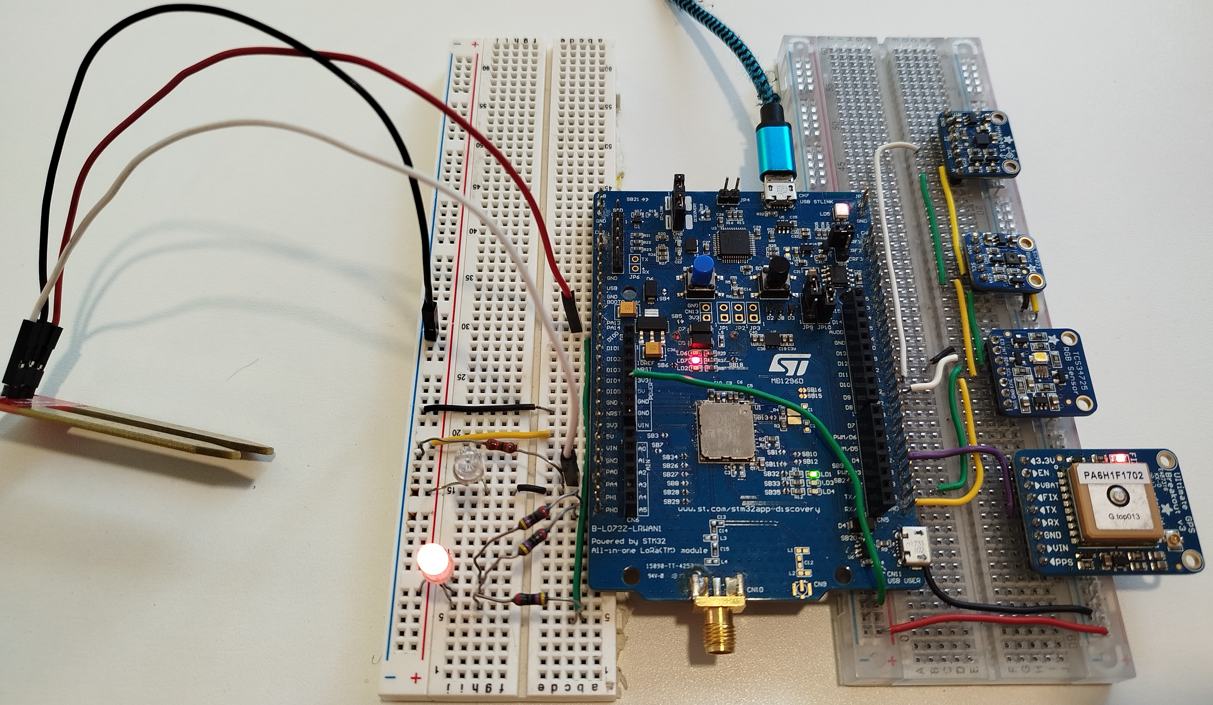
\includegraphics[width=1\textwidth]{images/1/sistema.png}
    \caption{Final solution developed}
    \label{fig:solutionIntro}
\end{figure}
\clearpage
\fancyhead[R]{\textit{REQUIREMENTS ANALYSIS}}
\section{REQUIREMENTS ANALYSIS}
\subsection{Specifications required and implemented}

This section presents in the next tables the list of requirements needed to implement, as well as the implementation status for each specification.
\vspace{2\baselineskip}
\begin{table}[H]
    \begin{center}
        \begin{tabular}{|p{0.1\textwidth} | p{0.7\textwidth} | p{0.15\textwidth}|}
            \hline
            \textbf{Req. ID} & \textbf{Requirement description} & \textbf{Implemented}\\
            \hline
            SR1 & The temperature in the range of -10ºC to 50ºC. Accuracy to one tenth of a degree. & Y\\
            \hline
            SR2 & The relative humidity in the range of 25\%HR to 75\%HR. Accuracy to one tenth of a percent. & Y\\
            \hline
            SR3 & Ambient light in \%, corresponding 0\% to total darkness and 100\% to maximum light. Accuracy to one tenth of a percent. & Y\\
            \hline
            SR4 & Soil moisture in \%, corresponding 0\% to total dryness and 100\% to maximum moisture. Accuracy to one tenth of a percent. & Y\\
            \hline
            SR5 & Colour of one leaf of the plant. The four associated parameters are clear, red, green, and blue values. & Y\\
            \hline
            SR6 & The global location of the plant should be registered. The GPS module also offers the current time (only time, the date is optional), that will be used to timestamp all the measurements taken by the system. & Y\\
            \hline
            SR7 & The acceleration of the plant. At least the three axes (X, Y and Z) values should be monitored. & Y\\
            \hline
            GR1 & The system must be robust and stable. & Y\\ %TODO ver que hago con esto
            \hline
            GR2 & Task partitioning and threads management should be stablished according to the requirements. & Y\\
            \hline
            GR3 & The system starts in TEST MODE and changes from one operating mode to the next one (TEST – NORMAL ADVANCED - TEST...) by pressing the blue button B1 on the B-L072Z-LRWAN1 board in a circular way. & Y\\
            \hline
        \end{tabular} 
    \end{center}
    \caption{General requirements implementation status}
    \label{ReqGeneral}
\end{table}

\vspace{2\baselineskip}

\begin{table}[H]
    \begin{center}
        \begin{tabular}{|p{0.1\textwidth} | p{0.7\textwidth} | p{0.15\textwidth}|}
            \hline
            \textbf{Req. ID} & \textbf{Requirement description} & \textbf{Implemented}\\
            \hline
            TM1 & Check connections and sensor management. & Y\\
            \hline
            TM2 & All of the required variables should be monitored every 2 seconds. & Y\\
            \hline
            TM3 & The system sends every 2 seconds all the measured values to the computer (using the USB virtual COM port of the B-L072Z-LRWAN1 board). & Y\\
            \hline
            TM4 & The RGB LED should be coloured in the dominant colour detected by the colour sensor. & Y\\
            \hline
            TM5 & In this mode, the LED1 of the B-L072Z-LRWAN1 board should be ON. & Y\\
            \hline
        \end{tabular} 
    \end{center}
    \caption{Test mode requirements implementation status}
    \label{ReqTest}
\end{table}

\begin{table}[H]
    \begin{center}
        \begin{tabular}{|p{0.1\textwidth} | p{0.7\textwidth} | p{0.15\textwidth}|}
            \hline
            \textbf{Req. ID} & \textbf{Requirement description} & \textbf{Implemented}\\
            \hline
            NM1 & All the required variables should be monitored with a cadence of 30s. & Y\\
            \hline
            NM2 & The system sends every 30 seconds all the measured values to the computer (using the USB virtual COM port of the B-L072Z-LRWAN1 board). & Y\\
            \hline
            NM3 & The system calculates the mean, maximum and minimum values of temperature, relative humidity, ambient light and soil moisture every hour. These values are sent to the computer when calculated. & Y\\
            \hline
            NM4 & The system calculates the dominant colour of the leave every hour. This means to calculate which colour has appeared as dominant more times during the last hour. This value is sent to the computer when calculated. & Y\\
            \hline
            NM5 & The system calculates the maximum and minimum values of the three axes (X, y and Z) of the accelerometer every hour. These values are sent to the computer when calculated. & Y\\
            \hline
            NM6 & The global location of the plant (coordinates) is sent to the computer every 30 seconds. This should include the GPS time (UTC) converted to local time. & Y\\
            \hline
            NM7 & Limits for every measured variable (temperature, humidity, ambient light, soil moisture, colour and acceleration) should be fixed. If the current values of the measured parameters are outside the limits, the RGB LED should indicate this situation using a different colour for every parameter. & Y\\
            \hline
            NM8 & In this mode, the LED2 of the B-L072Z-LRWAN1 board should be ON. & Y\\
            \hline
        \end{tabular} 
    \end{center}
    \caption{Normal mode requirements implementation status}
    \label{ReqNormal}
\end{table}
\subsection{Extra specifications implemented}
\begin{table}[H]
    \begin{center}
        \begin{tabular}{|p{0.1\textwidth} | p{0.7\textwidth} | p{0.15\textwidth}|}
            \hline
            \textbf{Req. ID} & \textbf{Requirement description} & \textbf{Implemented}\\
            \hline
            E1 & The date is also extracted from the GPS data. & Y\\
            \hline
            E2 & Compensation for the spectral response of the colour sensor is introduced. & Y\\
            \hline
            E3 & Automatic generation of the documentation with a Doxygen file and automatic publishing in a github pages. & Y\\
            \hline
        \end{tabular} 
    \end{center}
    \caption{Extra requirements implemented}
    \label{ReqExtra}
\end{table}
\clearpage
\fancyhead[R]{\textit{HARDWARE DESIGN}}
\section{HARDWARE DESIGN}
For this section and phase of the project, the next steps were done:
\begin{itemize}
    \item Analyzing the hardware elements.
    \item Analyze the connections needed.
    \item Select the pin connections for every element.
    \item Mount the system.
\end{itemize}
This approach led to a faster design of the solution.
\subsection{Hardware elements}
For the development of the project, all the hardware elements were identified and studied to obtain information of all the possible utilities that the system could use.
\begin{itemize}
    \item \textbf{DISCO-L072CZ-LRWAN1}\cite{DISCOL072CZLRWAN1Mbeda}: This embedded platform integrates the \texttt{STM32L072CZ}\cite{STM32L072CZUltralowpowerArm} cortex M0+ chip. This platform 
    focuses on the connectivity of the system. It provides:
    \begin{itemize}
        \item 192KB of flash memory.
        \item 20KB of RAM.
        \item USER and RESET button.
        \item \acrshort{i2c} and \acrshort{uart} connections.
        \item 16 bit timers along with LowPower timers.
        \item Low Power modes.
        \item A SX1276 transceiver that will be used to implement LoraWan communications on the next subject.
    \end{itemize}
    \item \textbf{I2C Accelerometer}\cite{MMA8451Q1a}: This sensor by Freescale, integrated by Adafruit\cite{DownloadsAdafruitMMA8451} offers 
    a 14 bit triple-axis accelerometer, as well as a  interruptions for events such as freefall and motion detection, transient detection, orientation changes and tap detections.\newline
    It also provides low power modes and deep configuration for sensibility.
    \item \textbf{I2C Color Sensor}\cite{TCS34725}: This chip by \acrfullr{taos} is integrated in a breakout board by Adafruit\cite{RGBColorSensor}. It consist on a 3 by 4 photodiode array with configurable integrators. 
    \newline It provides readings for clear, red, green and blue values in a 16 bit format. It also provides configuration for integration time, automatic readings and configurable interruptions for limits on the clear value.
    \item \textbf{I2C Temperature and Humidity Sensor}\cite{Support_Documents_TechnicalDocs_Si7021A20}: This chip by Silicon Labs is integrated in a breakout board by Adafruit. It allows readings of relative humidity and temperature of the air.
    \item \textbf{UART GPS}\cite{GlobalTopFGPMMOPA6HDatasheetV0A}: This GPS sensor with the integration from Adafruit\cite{gpsDownloadsAda} provides real time information about location following the \acrfullr{nmea} data standard.
    \item \textbf{SEN-13322 Analog Soil Moisture Sensor}\cite{SparkFunSoilMoisture}: This sensor by SparkFun allows to read the moisture level between the two pads.
    \item \textbf{RGB Led}: A common anode RGB led.
    \item \textbf{Phototransistor}\cite{HW5P1_2015__1_}: This element allows for the reading of the brightness in the environment.
\end{itemize}
\clearpage
\subsection{Block Diagram}
To design the solution, the diagram in \autoref{fig:proposedBlock} identifies the main blocks and hardware interfaces needed. The left side and the GPS include 5V powered elements, and the right side contains 3.3V elements.
\begin{figure}[H]
    \centering
    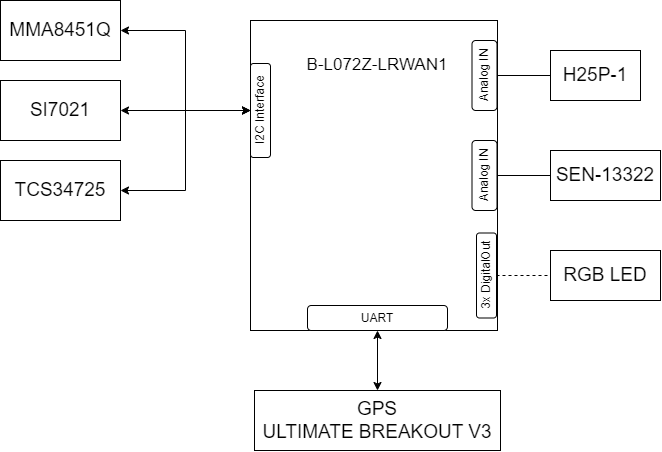
\includegraphics[width=0.6\textwidth]{images/3/General.drawio.png}
    \caption{Block identification for the hardware connections}
    \label{fig:proposedBlock}
\end{figure}

Next, the selection of the connections to the L072CZ were done in the next order: \acrshort{i2c}, \acrshort{uart}, analog connections and finally DigitalOut connections. It is important to note that, as we needed to indicate the working mode with the board leds, we can't 
use the pins connected directly to those elements.
\begin{itemize}
    \item For the I2C, the \acrfullr{mcu} offers 3 options, I2C1,I2C2 and I2C3, being the second one the worst in terms of capabilities.For this system and this use case, I2C1 was selected because, as seen in \autoref{fig:communications}, its the interface with less conflicts.
    \item For the Serial interface to communicate with the GPS, the options are \texttt{USART1}, \texttt{USART2}, \texttt{USART4} and \texttt{USART5}, with the last two having less capabilities. In this case, the L072CZ really only offers the first two, but the \texttt{USART2} 
    is used as a virtual COM port with the ST-Link. The selection was the \texttt{USART1}, also, as can be seen in \autoref{fig:communications}, it has the least conflicts of all.
    \item For the analog sensors, the \texttt{PA\_0} and \texttt{PA\_4} pins were selected, as we only need two Analog IN connections.
\end{itemize}

\begin{figure}[H]
    \centering
    \begin{subfigure}[t]{0.45\textwidth}
        \centering
        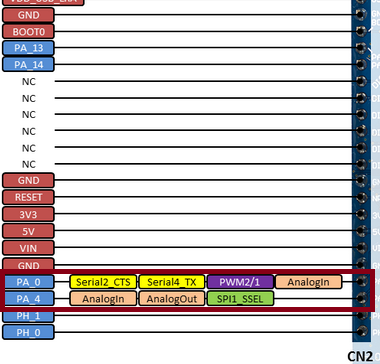
\includegraphics[width=0.66\textwidth]{images/3/Analog.png}
        \caption{Analog selection}
    \end{subfigure}
    \begin{subfigure}[t]{0.45\textwidth}
        \centering
        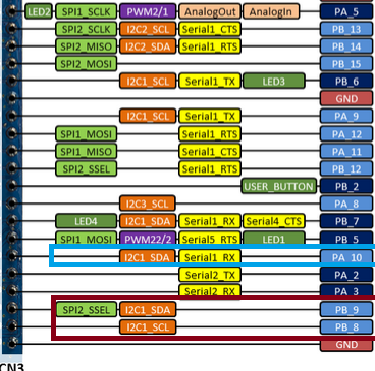
\includegraphics[width=0.66\textwidth]{images/3/I2CSerial.png}
        \caption{I2C and UART selection}
    \end{subfigure}
    \caption{Communication interfaces selection}
    \label{fig:communications}
\end{figure}
\clearpage
At last, the final DigitalOut connections were defined. The final connections for every element are defined in the next tables.
\begin{table}[H]
    \begin{center}
        \begin{tabular}{|p{0.20\textwidth} | p{0.20\textwidth} | p{0.20\textwidth}| p{0.20\textwidth}|}
            \hline
            \textbf{Sensor} & \textbf{Sensor Pin} & \textbf{L072CZ connector} & \textbf{L072CZ Pin name}\\
            \hline
            H25P-1 & SIG & CN2\_24 & PA\_4 \\
            \hline
            SEN-13322 & SIG & CN2\_23 & PA\_0 \\
            \hline
            RGB Led & RED & CN2\_23 & PA\_0 \\%TODO
            \hline
            RGB Led & GREEN & CN2\_23 & PA\_0 \\
            \hline
            RGB Led & BLUE & CN2\_23 & PA\_0 \\
            \hline
             & GND & CN2\_17 & GND \\
            \hline
             & VCC & CN2\_19 & +3.3V \\
            \hline
        \end{tabular}
    \end{center}
    \caption{Connections for the 3.3V elements}
    \label{Connections3}
\end{table}
\begin{table}[H]
    \begin{center}
        \begin{tabular}{|p{0.20\textwidth} | p{0.20\textwidth} | p{0.20\textwidth}| p{0.20\textwidth}|}
            \hline
            \textbf{Sensor} & \textbf{Sensor Pin} & \textbf{L072CZ connector} & \textbf{L072CZ Pin name}\\
            \hline
            TCS34725 & LED & CN3\_13 & PA\_9 \\
            \hline
            TCS34725 & INT & CN3\_15 & PA\_11 \\
            \hline
            GPS & SerialTX & CN3\_26 & PA\_10 \\
            \hline
            MMA8451Q & I2 & CN3\_14 & PA\_12 \\
            \hline
             & SCL & CN3\_25 & PB\_8 \\
            \hline
             & SDA & CN3\_24 & PB\_9 \\
            \hline
             & GND & CN3\_26 & GND \\
            \hline
             & VCC & CN2\_20 & +5V \\
            \hline
        \end{tabular} 
    \end{center}
    \caption{Connections for the 5V elements}
    \label{Connections5}
\end{table}


\clearpage
\fancyhead[R]{\textit{SOFTWARE}}
\section{SOFTWARE}

\subsection{Description of the implementation}
The solution is implemented with a \acrfullr{fsm} with three states, starting from a TEST mode and switching to the next with the USER button of the L072CZ. A common factor of these states is that in all of them, all the data from the sensors need to be obtained.

To solve the need for asynchronous data obtention from the sensors, the solution is based on threads and queues. There are three threads:
\begin{itemize}
    \item Main thread with the \acrshort{fsm}.
    \item I2C thread.
    \item GPS thread.
\end{itemize}

These thread are signalized to wake up when new measurements are needed by the \acrshort{fsm}. When all the information is collected, the information goes to the main thread through a Mbed-OS queue. When all the necessary 
information is obtained, the main thread sends the new data to the computer and waits a set amount of time to start the process again.
\subsection{Module, threads and communications design}
To make the design modular, each hardware element is implemented in a single module, with a \texttt{.cpp} and a \texttt{.h} file.

Considering the asynchronous nature of some of the sensors, the i2c sensors were implemented in an independent thread and the GPS in another thread. In the , the final module design as well as the threads implemented 
can be seen in \autoref{fig:moduleDiagram}.
\begin{figure}[H]
    \centering
    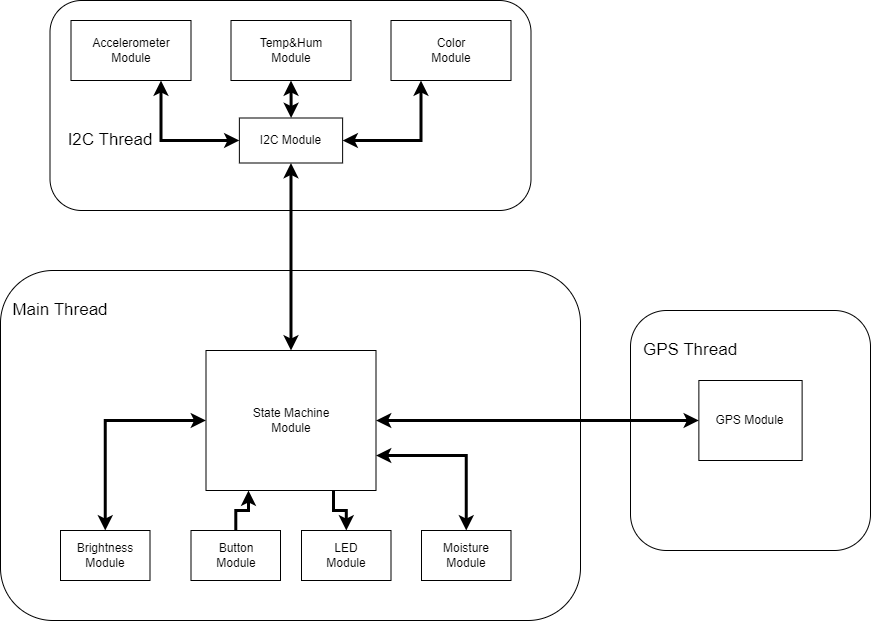
\includegraphics[width=0.9\textwidth]{images/4/softdiagram.png}
    \caption{Module diagram of the software and threads}
    \label{fig:moduleDiagram}
\end{figure}

For the communications from the control to the \acrshort{i2c} and the GPS, there was only need to indicate to the \acrshort{i2c} and GPS threads to launch all the necessary measurements on demand, so in this case signals were used.
For the data flowing from the sensors to the control module, as signals in a processor are limited(in our case 32 bit register for signals), a queue was used.

A queue is a thread safe mechanism of low level that implements a FIFO buffer with a in endpoint and an out endpoint. Any process can insert new data into the queue with a blocking call and the same can be done to extract the data. Finally, the data 
inside the queue is managed by the queue itself(at least in the implementation in Mbed-OS).

To reduce the memory usage, only one queue was defined for the whole system. With this done, extra logic was needed to differentiate messages from different sensors, so a message structure was defined like a pseudo-protocol. This can be seen in the \hyperref[appendix]{appendix}.

\subsection{State machine module}
At the start of the system, the main calls for the initialization of all the modules. This is important because the creation of the I2C and GPS threads take some time. When this is done, the main initializes the state machine 
and enters a loop to do a cycle of the state machine.

The state machine includes two timeouts that are configured for each state, depending on the needs.
\begin{itemize}
    \item The first timeout is configured as the time needed between sending the information to the computer.
    \item For the second timeout, the configuration is to make it generate an interruption \texttt{400 ms} earlier. When this happens, the controller sends signals for every thread. This signal enforces the reading of new 
    measurements.
\end{itemize}
When the signals are sent, the main thread is sent to sleep \texttt{400 ms}, at that time, it wakes up and analyzes all the data that has been sent to the queue. This time was selected as a time to let the other threads collect all the necessary data.

When all the messages are collected, the data is processed depending on the state of the system:
\begin{itemize}
    \item TEST mode: as the requirements specify, the data is formatted and sent to the computer as in \autoref{fig:testSerial}. Depending on the highest color component, the RGB led changes accordingly.
    \begin{figure}[H]
        \centering
        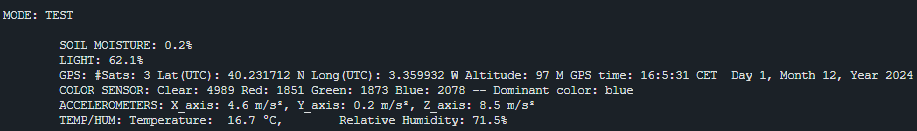
\includegraphics[width=0.9\textwidth]{images/4/TestSerial.png}
        \caption{Information sent to the computer in the TEST mode}
        \label{fig:testSerial}
    \end{figure}
    \clearpage
    \item NORMAL mode: as the requirements specify, the time the messages are read, maximum values and mean values are calculated, as well as situations like extreme moisture.
    
    All the limitations are in the \autoref{Limits}.

    \begin{table}[H]
        \begin{center}
            \begin{tabular}{|p{0.20\textwidth} | p{0.20\textwidth} | p{0.20\textwidth}| p{0.20\textwidth}|}
                \hline
                \textbf{Parameter} & \textbf{High limit} & \textbf{Low limit} & \textbf{Led color}\\
                \hline
                Temperature & 35 & 10 & red \\
                \hline
                Humidity & 75 & 25 & blue \\
                \hline
                Brightness & 80 & 10 & Yellow \\
                \hline
                Moisture & 85 & 5 & Purple \\
                \hline
                Color & Blue &  & White \\
                \hline
            \end{tabular}
        \end{center}
        \caption{Limits defined for the parameters in the NORMAL mode}
        \label{Limits}
    \end{table}

    All of this information is sent to the computer, and when one hour has passed, the maximum and mean values are also sent. The format is presented in \autoref{fig:normalSerial}.
    \begin{figure}[H]
        \centering
        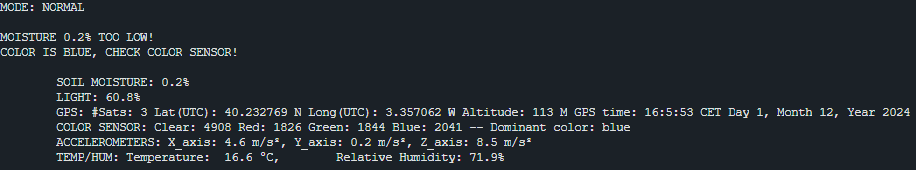
\includegraphics[width=0.9\textwidth]{images/4/NormalSerial.png}
        \caption{Information sent to the computer in the NORMAL mode}
        \label{fig:normalSerial}
    \end{figure}

    \item ADVANCED mode: this mode is presented and described in it's own chapter.%TODO meter label y hyperef
\end{itemize}

Finally, the USER button allows for switching modes in a circular way. When this button is pressed:
\begin{enumerate}
    \item The timeouts are re-configured.
    \item The led of the board that is on changes to indicate the new state.
    \item The RGB led is turned off.
    \item The thread waits \texttt{400 ms} for any new messages from the other threads, in order to empty the queue for the new state.%TODO hablar de este problema.
\end{enumerate}

As a final note, as this state machine is working under the main thread of Mbed-OS, no changes were done to the stack or any other property of this thread.
\clearpage
\subsection{I2C module}

The \acrshort{i2c} module controls the measurement of the accelerometer, temperature and humidity and color sensors.

As there are three different sensors with different requirements, at the initialization of the I2C thread, all the sensors are started sequentially, using a global I2C object. It must be noted that as all the sensors 
support it, the I2C is used with a frequency of \texttt{400 kHz}.

For the initialization, the next steps are done:
\begin{itemize}
    \item \textbf{Initialization of the accelerometer}: first the accelerometer is reseated, when this finish, the dynamic configuration is set to 8G, this is because the use case doesn't need that much high sensibility.
    \item \textbf{Initialization of the color sensor}: for the color sensor, the dataset specifies a different approach with a command register. In this case, this sensor is configured to remove any wait state, this is done because 
    the sensor has a limit of wait time less that 30 seconds, so the readings are done on demand, this is by turning on and off the sensor. Lastly, the sensor is configured with an integration time of \texttt{154 ms}.
\end{itemize}

When all the configuration is done, the thread enters a loop where it waits for an \texttt{I2C\_SIGNAL} from the state machine. Once this happens, the flag is cleared and the next steps happen:
\begin{enumerate}
    \item Reading of the accelerometer data, conversion of the data and queue acceleration message sent.
    \item Powering the color sensor, waiting for the integration time and reading of the data to send the color message. Power off the sensor.
    \item Force a reading of humidity and temperature, converting values as told in the dataset\cite{Support_Documents_TechnicalDocs_Si7021A20}.
\end{enumerate}

To finalize, the thread goes back to wait for another signal from the state machine.
\clearpage
\subsection{GPS module}
The GPS module implements the GPS thread and focuses on obtaining and parsing the data from the GPS chip.

The GPS is constantly sending data to the serial connection in a baud rate of \texttt{9600}. To read this data, when the thread wakes from a \texttt{GPS\_SIGNAL}, the thread is constantly reading the characters obtained in the \acrshort{uart} and adding them to a 
buffer. If the next character is a new line character, the buffer is sent to the parse\_gps\_sentence function.

For this parsing, as the system only needs the location, time and data, the parsing is only done to specific sentences of the \acrshort{nmea} data format in \autoref{fig:nmeaSentences}.
\begin{figure}[H]
    \centering
    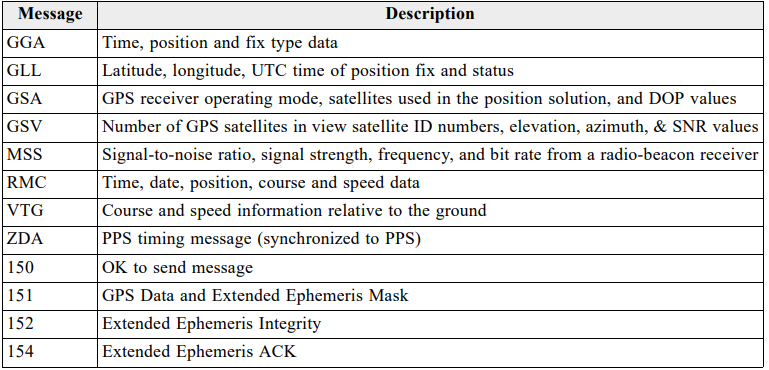
\includegraphics[width=0.9\textwidth]{images/4/nmea.png}
    \caption{NMEA possible sentences\cite{NMEAReferenceManual}}
    \label{fig:nmeaSentences}
\end{figure}
In this use case, the GPS thread only searches for:
\begin{itemize}
    \item \textbf{GGA}: contains the information about the actual time, latitude, longitude, altitude and number of satellites detected.
    \item \textbf{RMC}: contains information about the actual time, the actual date and other data that the system doesn't use.
\end{itemize}
To parse the sentences, the function \texttt{strncmp} was used to analyze the sentence type and \texttt{sscanf} to parse all the information like a pseudo-regex.

When both sentences are found, the message for the queue is built and inserted, finally, the GPS thread goes back to wait for a new signal from the state machine.

\clearpage
\subsection{Code size}
For the code size of the project, the information resulting from the compilation in Mbed Studio is presented in the next figures. It must be noted that no changes to the default compilation profiles were done.
\begin{figure}[H]
    \centering
    \begin{subfigure}[t]{0.45\textwidth}
        \centering
        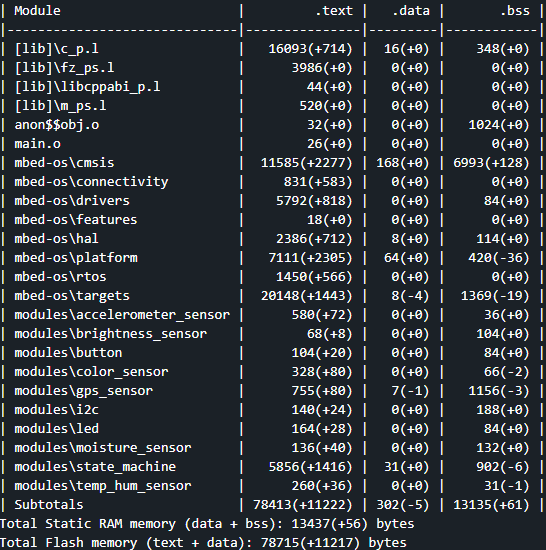
\includegraphics[width=0.95\textwidth]{images/4/Debug.png}
        \caption{Debug compilation}
    \end{subfigure}
    \begin{subfigure}[t]{0.45\textwidth}
        \centering
        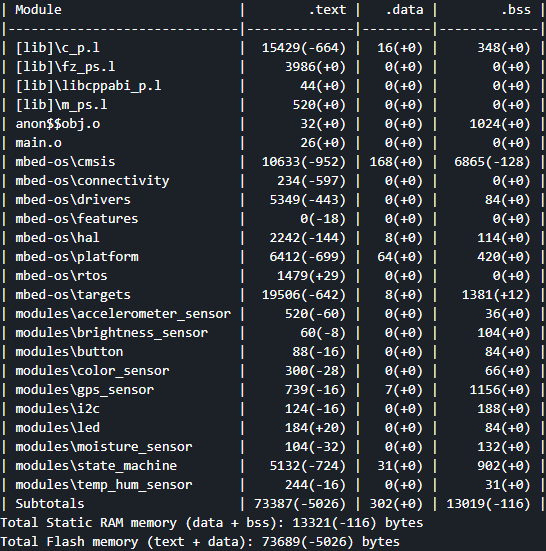
\includegraphics[width=0.95\textwidth]{images/4/Develop.png}
        \caption{Develop compilation}
    \end{subfigure}
    \begin{subfigure}[t]{0.45\textwidth}
        \centering
        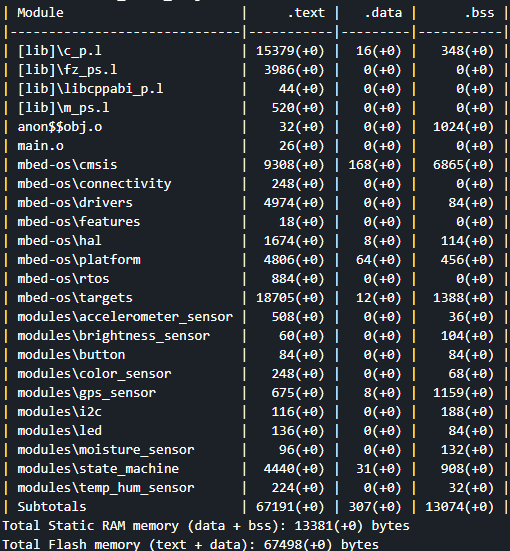
\includegraphics[width=0.95\textwidth]{images/4/Release.png}
        \caption{Release compilation}
    \end{subfigure}
    \caption{Code size and module size for every compilation profile}
    \label{fig:compilation}
\end{figure}

The most heavy modules in terms of size were:
\begin{enumerate}
    \item The state machine with 476 lines of code.
    \item The GPS with 86 lines of code, but with a parsing of a string, which needs lot of resources.
\end{enumerate}

\clearpage
\fancyhead[R]{\textit{ADVANCED MODE IMPLEMENTATION}}
\section{ADVANCED MODE IMPLEMENTATION}
\clearpage
\fancyhead[R]{\textit{PROBLEMS DETECTED AND SOLUTIONS IMPLEMENTED}}
\section{PROBLEMS DETECTED AND SOLUTIONS IMPLEMENTED}
This chapter describes problems that appeared during the development of the project as well as solutions implemented.
\subsection{Debug mode}
When trying to work with the debug mode of Mbed Studio, and in an early version of the project, the debugger wasn't launching. The error can be seen in the next figure.
\begin{figure}[H]
    \centering
    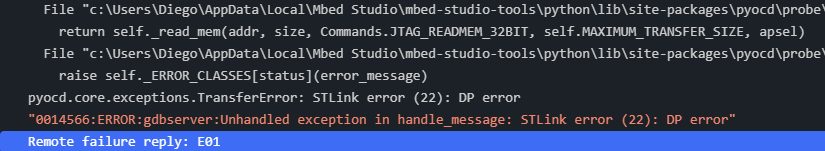
\includegraphics[width=0.8\textwidth]{images/6/Debug Problem.png}
    \caption{Debug error}
    \label{fig:debugProblem}
\end{figure}
As the project involved multiple modules, communication interfaces and threads. Some time was spent understanding the error and getting the debugger to work.

After research and trial and error. The solution was found. The L072CZ connects the \texttt{PA\_13} and \texttt{PA\_14} pins directly to the SW debugger of the ST Link as presented in the \autoref{fig:debugPins}. 
\begin{figure}[H]
    \centering
    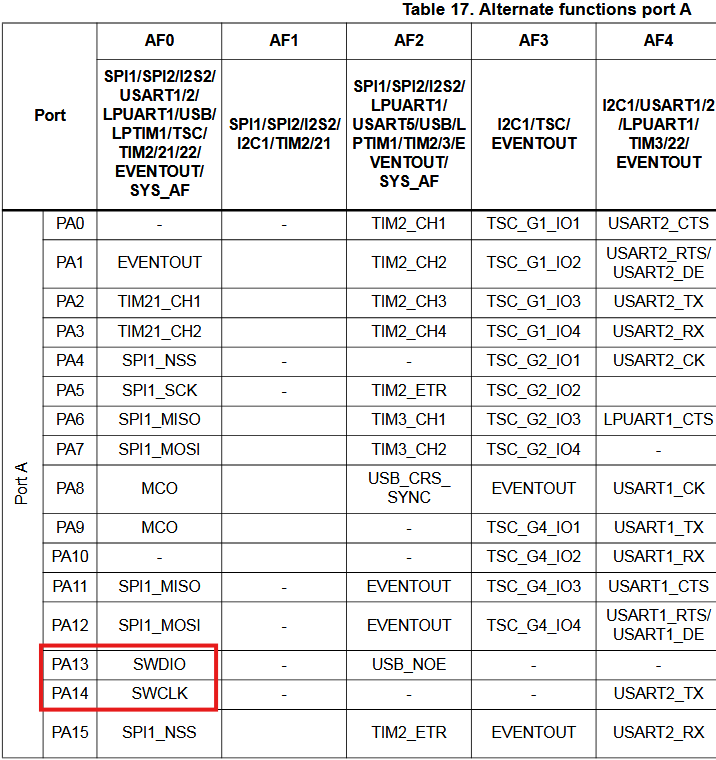
\includegraphics[width=0.6\textwidth]{images/6/DebugPins.png}
    \caption{Pins used by the SW debugger}
    \label{fig:debugPins}
\end{figure}
When the RGB Led was started, the alternate function of the pin is overwritten, and the connection to the debugger is lost. To solve this, a macro was defined in the system, that can be commented and allow the RGB led module to work with all the colors.

\subsection{Problems with the color sensor}
The color sensor was configured to implement the requirements of the advanced mode in regards to the interruptions generation. The configuration was properly validated with a logical analyzer.

When everything was configured, no observable change in the logical level of the interrupt pin was seen.

To see the problem in a modular way, an external implementation\cite{TCS3472_I2CClasswhich} of an interface to the sensor was used. When trying to enable the interruptions, the code returned a 0, indicating that 
a problem had ocurred.
\subsection{Problems with the accelerometer}
When working with the accelerometer, the data obtained wasn't being read properly. When inspected with the logical analyzer, the data that was being sent back to the \acrshort{mcu} was fixed. This can be seen in the next figure.
\begin{figure}[H]
    \centering
    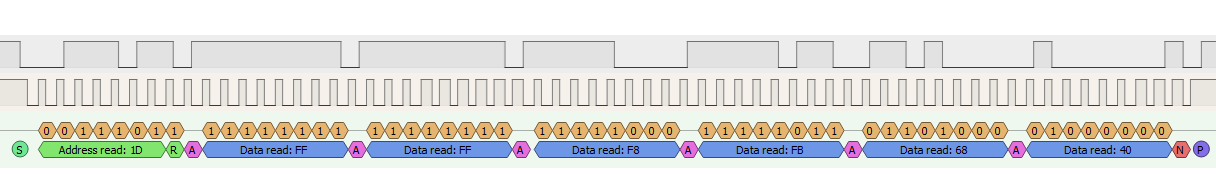
\includegraphics[width=0.9\textwidth]{images/6/accProblem.png}
    \caption{Accelerometer fixed data without repeated start}
    \label{fig:accProblems}
\end{figure}
After some research and, as vaguely indicated by the dataset\cite{MMA8451Q1a}, the sensor expects repeated start between write and read operations.
\subsection{Fault problem}
When implementing and testing the GPS, and in the final week, some HardFaults were seen in the project. After talking with the teachers of the subject, the main suspect of this problem were 
the change done in the default stack size of the Mbed-OS threads. In this case, one of the main possible conflict point is the GPS thread.

As the GPS thread performs parsing on strings, the amount of memory needed by the thread is more than expected, to solve this, more stack size was assign to the GPS thread.
\clearpage
\fancyhead[R]{\textit{TESTING AND VALIDATION}}
\section{TESTING AND VALIDATION}
\clearpage
\fancyhead[R]{\textit{DOCUMENTATION}}
\section{DOCUMENTATION}
As this project integrates different kinds of elements and software modules and all the design would be used for next subjects, it was decided that some of the efforts were going to be allocated on generating 
good documentation of the code.

To approach this, doxygen\cite{DoxygenGettingstarted} was used. Doxygen defines both the standard and an application to generate documentation in a Javadoc style in both HTML and LaTex documents.

All the documentation in the code was defined following the doxygen specifications. Lastly, a Doxyfile configuration file is generated considering the needs of the documentation. This created the documentation files 
but two problems were observed:
\begin{enumerate}
    \item The default HTML documentation feels old, so a open style for Doxygen called "doxygen-awesome-css"\cite{jotheprodoxygenawesomecss} was used. This led to a much clean documentation as in the \autoref{fig:doxyStyle}.
    
    \begin{figure}[H]
        \centering
        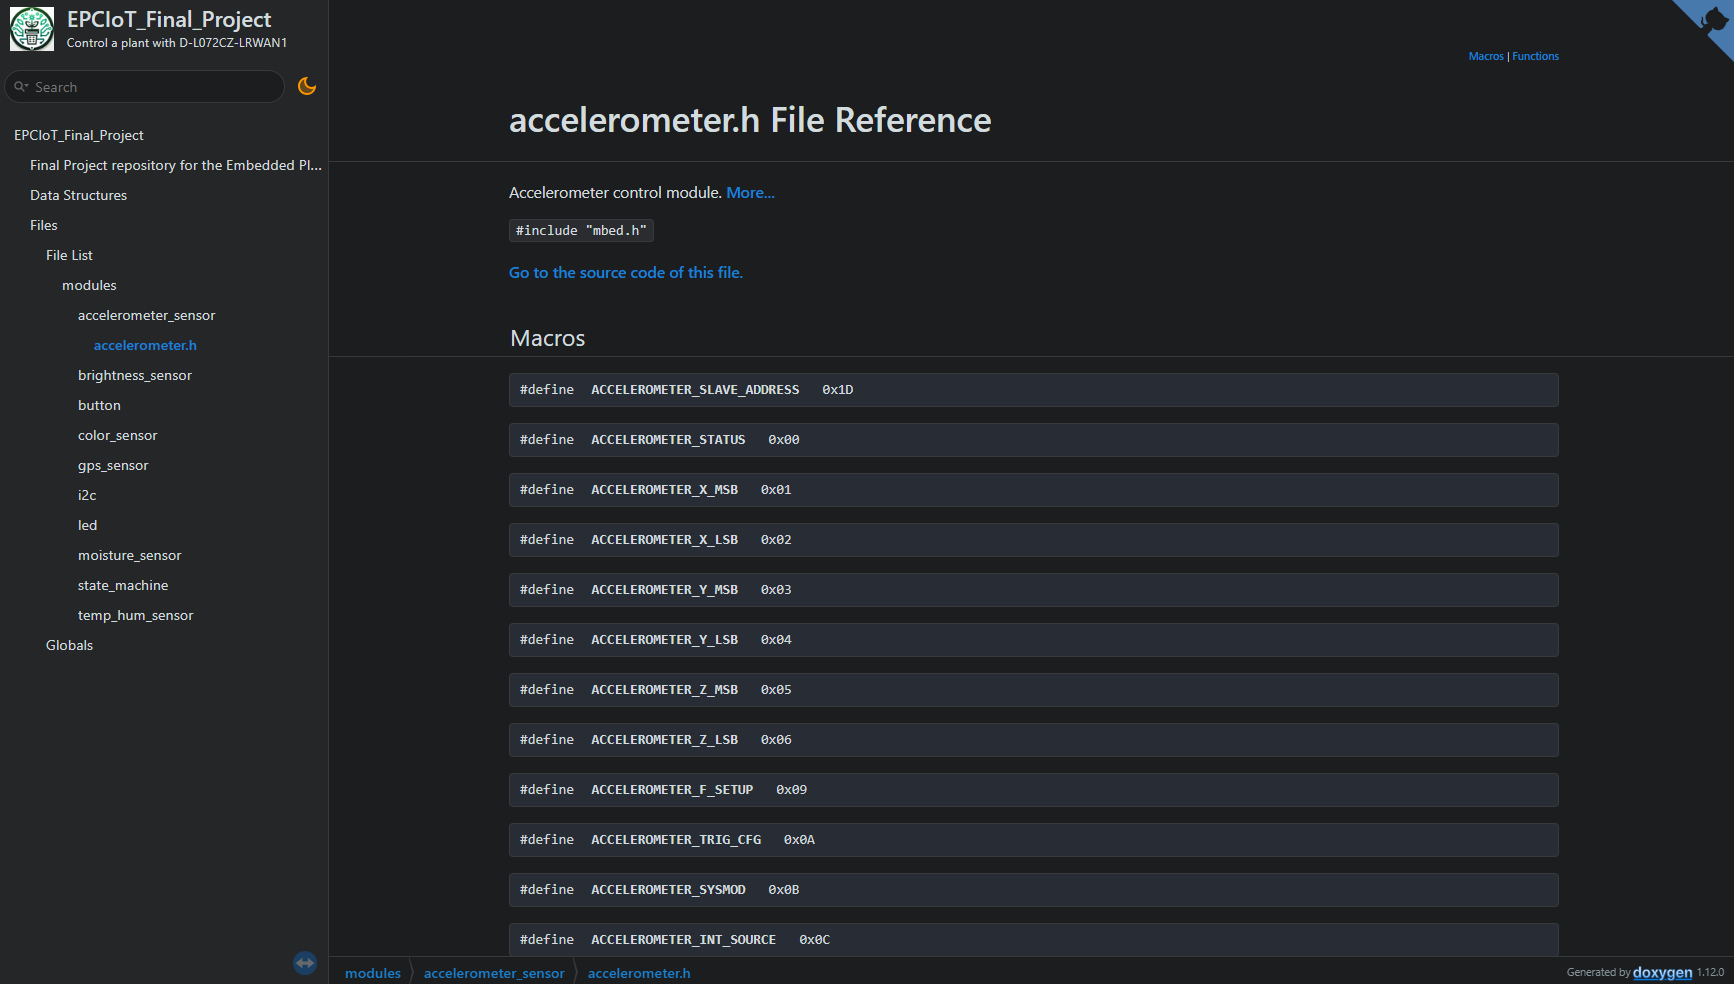
\includegraphics[width=0.8\textwidth]{images/8/doxy.png}
        \caption{Final documentation with the modified Doxygen}
        \label{fig:doxyStyle}
    \end{figure}

    \item As more functionalities were being added, the documentation needed to be re-generated. To solve this, a GitHub workflow was configured to auto-generate and auto-publish the generated HTML with an action in a branch of the repository. With GitHub pages, 
    the automatic deployment was configured.\newline The final result is available here: \url{https://ryvenkappa.github.io/EPCIoT_Final_Project/}
\end{enumerate}

\clearpage
\fancyhead[R]{\textit{RESULTS}}
\section{RESULTS}

The project was successfully implemented following the requirements specified. Also, the advanced mode was implemented and validated, following the requirements told by the teachers of the subject.

Also, for this subject, Doxygen was learnt and implemented to generate the documentation of the project. This was combined with GitHub actions.

The final public repository is available at: \url{https://github.com/RyvenKappa/EPCIoT_Final_Project}.




\clearpage
\fancyhead[R]{\textit{REFERENCES}}
\printbibliography[title={REFERENCES}, heading=bibnumbered]
\clearpage
\fancyhead[R]{\textit{APPENDIX}}
\section{APPENDIX: Control message structures}
\lstinputlisting[caption={Control.h}, label={lst:myfile}]{control.h}
\end{document}